\chapter{11 октября}

\textcolor{red}{Лекция ещё не записана.}

\begin{remark}
    Следующий материал был рассказан на практике 13 октября.
\end{remark}

\subsection{Распределение Коши}

Пусть дан источник некоторого излучения в точке \((0, 1)\), который равномерно посылает лучи во все стороны.

Случайная величина \(\xi\) --- точка пересечения луча с осью \(OX\).

Найти \(F_\xi(x), f_\xi(x), \E \xi\).

\begin{figure}[h]
    \centering
    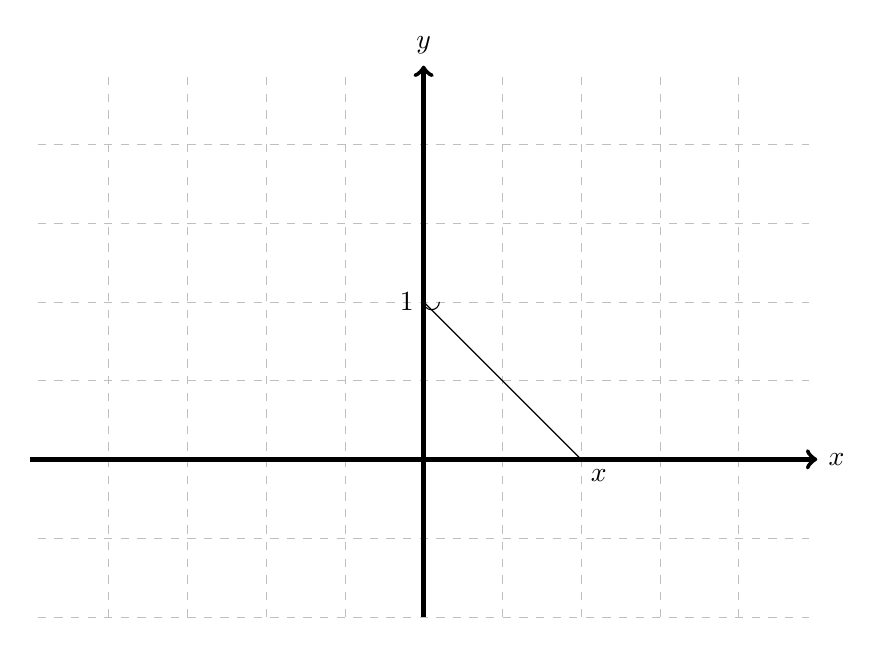
\begin{tikzpicture}
        \draw[help lines, color=gray!50, dashed] (-4.9,-2) grid (4.9,4.9);
        \draw[->,ultra thick] (-5,0)--(5,0) node[right]{$x$};
        \draw[->,ultra thick] (0,-2)--(0,5) node[above]{$y$};
        \draw (0, 2) node[left] {1} -- (2, 0);
        \node[below right] at (2, 0) {\(x\)};
        \draw (0, 2) arc (180:360:0.1);
    \end{tikzpicture}
    \caption{Источник}
\end{figure}

\[F_\xi(x) = P(\xi < x) = P(\xi < 0) + P(0 < \xi < x) = 0.5 + \frac{1}{\pi} \arctg x\]
\[f_\xi(x) = F_\xi'(x) = \frac{1}{\pi} \frac{1}{x^2 + 1}\]
\[\E \xi = \int_{ - \infty }^{ + \infty } x f_\xi(x) = \int_{ - \infty }^{ + \infty } x \frac{1}{\pi} \frac{1}{x^2 + 1} dx = \frac{1}{2 \pi} \ln(1 + x^2) \Big|_{ - \infty }^{ + \infty}, \nexists\]

Пусть теперь источник сдвинут на \(\theta\) по оси \(x\). Тогда \(f_\xi(x) = \frac{1}{\pi (1 + (x - \theta)^2)}\). Попробуем оценить \(\theta\). \(\overline{X}\) не работает, т.к. оно убежит на бесконечность: \(\E \frac{S_n}{n} = \E X\). Оценим с помощью медианы. По симметрии \(\theta = \mathrm{Me} \xi\).

\[\mathrm{Me}^* = \begin{cases}
        X_{(k + 1)},                     & n = 2k + 1 \\
        \frac{X_{(k)} + X_{(k + 1)}}{2}, & n = 2k
    \end{cases}\]

\begin{theorem}
    Если \(f(\mathrm{Me}) \neq 0\), то \(\mathrm{Me}^* \xrightarrow{P} \mathrm{Me}\), причём сходится со скоростью \(\frac{1}{\sqrt{n}}\).
\end{theorem}

В целом при большом числе выбросов медиана помогает. Например, оценивать зарплату нужно по медиане, а не по среднему.

У медианы также есть свои недостатки: она сходится медленнее, чем выборочное среднее --- эффективность обычно ниже на 20-30\%, но бывают и случаи хуже.

Есть и другие оценки, например \textbf{усечённое среднее}. Выкидываются наименьшие и наибольшие \(k\) точек и считается выборочное среднее:
\[\frac{\sum\limits_{i= k + 1}^{n - k} X_{(i)}}{n - 2k}\]
Несложно заметить, что это нечто промежуточное между выборочным средним и медианой --- если \(k = 0\), то получаем выборочное среднее, если \(k = \frac{n - 1}{2}\), то получаем медиану.

Другой пример: составим по исходной выборке выборку объема \(\frac{n(n - 1)}{2}\), состоящую из \(\frac{X_i + X_j}{2}, 1 \leq i,j \leq n\). \textbf{Среднее Уолша} --- медиана этой выборки. У этой оценки эффективность падает на \(\approx 12\%\) относительно выборочного среднего.

\begin{exercise}
    Дано \(n\) призывников с вероятностью болезни \(p = 0.01\). Разбиваем призывников на группы по \(k\) человек в группе. Считаем, что \(n \divided k\), т.е. групп \(\frac{n}{k}\). В каждой группе:
    \begin{itemize}
        \item Если суммарный результат отрицательный, то \(1\) анализ.
        \item Иначе \(k + 1\) анализ.
    \end{itemize}

    Найти оптимиальное значение \(k\) и среднее значение числа анализов.
\end{exercise}
\begin{solution}
    \(\xi_i\) --- число анализов в \(i\)-той группе.

    \[P(\xi_i = 1) = (1 - p)^k \quad P(\xi_i = k + 1) = 1 - (1 - p)^k\]
    \[\E \xi_i = (1 - p)^k + (k + 1)(1 - (1 - p)^k) = k + 1 - k(1 - p)^k\]
    \[\xi = \frac{n}{k} \cdot \xi_i\]
    \[\E \xi = n\left(1 + \frac{1}{k} - (1 - p)^k\right) = f(k)\]
    Т.к. \(p\) мало, пусть оно \(p \to 0\). \((1 - p)^k \sim 1 - pk\).
    \[f(k) \sim n \left(\frac{1}{k} + pk\right)\]
    \[f'(k) = n \left( - \frac{1}{k^2} + p \right) = 0\]
    \[k = \frac{1}{\sqrt{p}} = 10\]
    \[\E \xi \approx n \left(\frac{1}{10} + 0.01 \cdot 10\right) = 0.2 n\]
\end{solution}
